\documentclass[twoside,10pt]{article}
%=================================================
% Basics
%=================================================
\usepackage{fixltx2e} % Makes \( \) equation style robust, among other
                      % things. Must be the first package.


% Makes ligatured fonts searchable and copyable in pdf readers
\usepackage{cmap} % Load before fontenc 

% Always include these font encodings in your document 
% unless you have a very good reason.
\usepackage[T1]{fontenc}
\usepackage[utf8]{inputenc}

\usepackage{verbatim}

%=============
% Fonts
%=============

\usepackage{lmodern} % Improved version of computer modern
\usepackage[scale=0.88]{tgheros} % Helvetica clone for sans serif font


\newcommand\hmmax{2} % Default is 3.
\newcommand\bmmax{2} % Default is 4.

\usepackage{bm} % boldmath must be called after the package
\providecommand{\mathbold}[1]{\bm{#1}}

%=============
% AMS Packages and fonts
%=============
\usepackage{amsmath,amsbsy,amsgen,amscd,amsthm,amsfonts,amssymb} 

%=============
% Margins and paper size
%=============
\usepackage[centering,top=1.5in,bottom=1.2in,left=1.4in,right=1.4in]{geometry}
\usepackage{parskip}


%=============
% Section headings
%=============
\usepackage[sf,bf,compact]{titlesec}

%=============
% Tables and lists
%=============
\usepackage{booktabs,longtable,tabu} % Nice tables
\setlength{\tabulinesep}{1mm}
\usepackage[font=small,margin=10pt,labelfont={sf,bf},labelsep={space}]{caption}

%=============
% Code output
%=============
% \usepackage{listings}
% \usepackage{minted}




\usepackage{enumitem}
\setitemize{itemsep=0pt} 
\setenumerate{itemsep=0pt}
\setlist{labelindent=\parindent,%  % Recommended by enumitem package
  font=\sffamily}


%=============
% Hyperlink colors
%=============
\usepackage[usenames,dvipsnames]{xcolor}
\definecolor{steelblue}{HTML}{A1BDC7}
\definecolor{orange}{HTML}{D98C21}
\definecolor{silver}{HTML}{B0ABA8}
\definecolor{rust}{HTML}{B8420F}
\definecolor{seagreen}{HTML}{2E6B69}
\definecolor{joshua}{HTML}{FBDC7F}
\definecolor{darksky}{HTML}{154c79}

\colorlet{steelblue}{silver!30!white}
\colorlet{darkorange}{orange!85!black}
\colorlet{darksilver}{silver!85!black}
\colorlet{darksteelblue}{steelblue!85!black}
\colorlet{darkrust}{rust!85!black}
\colorlet{darkseagreen}{seagreen!85!black}

\usepackage{url}
\usepackage[colorlinks=true]{hyperref}
\hypersetup{linkcolor=darkrust}    
\hypersetup{citecolor=darkseagreen}      
\hypersetup{urlcolor=darksilver}     

%=============
% Microtype
%=============
\usepackage[final]{microtype} 

%=====================
% Header
%=====================
% \usepackage{fancyhdr}
% \usepackage{nopageno} % Gets rid of page number at the bottom
% \fancyhf{} % Clear header style
% \renewcommand{\headrulewidth}{0.5pt} % remove the header rule
% \pagestyle{fancy}
% \fancyhead[LE,RO]{\textsf{\small \thepage}}
% 
% \setlength{\headheight}{14pt}
%=====================
% Fix delimiters
%=====================

% Fixes \left and \right spacing issues. See discussion at
% http://tex.stackexchange.com/questions/2607/spacing-around-left-and-right
\let\originalleft\left
\let\originalright\right
\renewcommand{\left}{\mathopen{}\mathclose\bgroup\originalleft}
\renewcommand{\right}{\aftergroup\egroup\originalright}

%=================================================
% Math macros
%=================================================

%=============
% Generalities
%=============
\usepackage{mathtools}
\mathtoolsset{centercolon}  % Makes := typeset correctly for definitions

%%% Equation numbering
%\numberwithin{equation}{section} 

%%% Annotations
\newcommand{\notate}[1]{\textcolor{red}{\textbf{[#1]}}}

%==============
% Symbols
%==============
\let\oldphi\phi
\let\oldeps\epsilon

\renewcommand{\phi}{\varphi}
\renewcommand{\epsilon}{\varepsilon}
\newcommand{\eps}{\varepsilon}

%==============
% Constants
%==============

% Set constants upright
\newcommand{\cnst}[1]{\mathrm{#1}}  
\newcommand{\econst}{\mathrm{e}}

\newcommand{\zerovct}{\vct{0}} % Zero vector
\newcommand{\Id}{\mathbf{I}} % Identity matrix
\newcommand{\onemtx}{\bm{1}}
\newcommand{\zeromtx}{\bm{0}}

%==============
% Sets
%==============
\providecommand{\mathbbm}{\mathbb} % In case we don't load bbm

% Reals, complex, naturals
\newcommand{\R}{\mathbbm{R}}
\newcommand{\C}{\mathbbm{C}}
\newcommand{\K}{\mathbbm{K}}
\newcommand{\N}{\mathbbm{N}}

%==============
% Probability
%==============
\newcommand{\Prob}{\operatorname{\mathbbm{P}}}
\newcommand{\Expect}{\operatorname{\mathbb{E}}}

%==============
% Vectors and matrices 
%==============
\newcommand{\vct}[1]{\mathbold{#1}}
\newcommand{\mtx}[1]{\mathbold{#1}}

\newcommand{\mrange}{\operatorname{range}}
\newcommand{\mnull}{\operatorname{null}}



\begin{document}

\title{CSE 6643 Homework 5}
\author{Karl Hiner, Spring 2023}
\date{}
\maketitle

\section{Power Method [30 pts]} 

We consider a matrix $\mtx{A}$ such that
\begin{equation} 
  \mtx{Q}^T \mtx{A} \mtx{Q} = \operatorname{diag}\left(\lambda_1, \ldots, \lambda_m\right),
\end{equation}
where $\mtx{Q}$ is orthogonal. We denote by $\vct{q}_i$ the $i$th column of $\mtx{Q}$. 

We now consider the power method and the sequence $\vct{\nu}^{(k)}$  defined as 
\begin{align}
  \vct{z}^{(k)} &= \mtx{A} \vct{\nu}^{(k - 1)} \\
  \vct{\nu}^{(k)} &= \vct{z}^{(k)} / \|\vct{z}^{(k)}\|_2,
\end{align}
where we assume that $\|\vct{\nu}^{(0)}\|_2 = 1$. Assume that we have $\theta_k$ such that 
\begin{equation}
  \cos(\theta_k) = \vct{q}_1^{T} \vct{\nu}^{(k)}
\end{equation}
with $\cos(\theta_{0}) \neq 0$.
Prove that 
\begin{equation}
  1 - \cos(\theta_k)^2 \leq \frac{1}{a_1^2} \sum \limits_{i = 2}^m a_i^2\left(\frac{\lambda_{i}}{\lambda_1}\right)^{2k}, \quad a_i = \vct{q}_i^T \vct{\nu}^{(0)} 
\end{equation}

\begin{align*}
  \cos(\theta_k) &= \vct{q}_1^{T} \vct{\nu}^{(k)}&\text{(given)}\\
  &= \vct{q}_1^{T} \frac{\mtx{A}^k \vct{\nu}^{(0)}}{\|\mtx{A}^k \vct{\nu}^{(0)}\|_2}&\text{(def. of power method)}\\
  &= \frac{\vct{q}_1^{T} \mtx{Q}\mtx{\Lambda}^k\mtx{Q}^T \vct{\nu}^{(0)}}{\|\mtx{Q}\mtx{\Lambda}^k\mtx{Q}^T \vct{\nu}^{(0)}\|_2}&\text{(def. of $\mtx{A}$)}\\
  &= \frac{\vct{q}_1^{T} \mtx{Q}\mtx{\Lambda}^k\vct{a}}{\|\mtx{Q}\mtx{\Lambda}^k\vct{a}\|_2}&\text{($\vct{a} \equiv \mtx{Q}^T\vct{\nu}^{(0)} \rightarrow a_i = \vct{q}_i^T \vct{\nu}^{(0)}$)}\\
  \cos(\theta_k)^2 &= \frac{\left(\vct{q}_1^{T} \mtx{Q}\mtx{\Lambda}^k\vct{a}\right)^2}{\|\mtx{Q}\mtx{\Lambda}^k\vct{a}\|_2^2}&\text{(square both sides)}\\
  &= \frac{\left(\vct{q}_1^{T} \mtx{Q}\mtx{\Lambda}^k\vct{a}\right)^2}{\left(\mtx{Q}\mtx{\Lambda}^k\vct{a}\right)^T\left(\mtx{Q}\mtx{\Lambda}^k\vct{a}\right)}&\text{(def. of 2-norm)}\\
  &= \frac{\left(\vct{q}_1^{T} \mtx{Q}\mtx{\Lambda}^k\vct{a}\right)^2}{\vct{a}^T\mtx{\Lambda}^k\mtx{Q}^T\mtx{Q}\mtx{\Lambda}^k\vct{a}}&\text{(apply transpose in den.)}\\
  &= \frac{\left(\vct{q}_1^{T} \mtx{Q}\mtx{\Lambda}^k\vct{a}\right)^2}{\mtx{\Lambda}^{2k}\vct{a}^T\vct{a}}&\text{(simplify den. $\mtx{Q}$ orth., $\mtx{\Lambda}$ diag.)}\\
  &= \frac{\left(\vct{q}_1^{T} \mtx{Q}\mtx{\Lambda}^k\vct{a}\right)^2}{\sum\limits_{i=1}^m{\lambda_i^{2k} a_i^2}}&\text{(expand den.)}\\
  &= \frac{\left(\vct{e}_1\mtx{\Lambda}^k\vct{a}\right)^2}{\sum\limits_{i=1}^m{\lambda_i^{2k} a_i^2}}&\text{($\vct{q}_1^T\cdot\vct{q}_1 = 1$, $\vct{q}_1^T\cdot\vct{q}_{i \neq 1} = 0$)}\\
  &= \frac{\lambda_1^{2k} a_1^2}{\sum\limits_{i=1}^m{\lambda_i^{2k} a_i^2}}&\text{(evaluate num.)}\\
  1 - \cos(\theta_k)^2 &= 1 - \frac{\lambda_1^{2k} a_1^2}{\sum\limits_{i=1}^m{\lambda_i^{2k} a_i^2}}&\text{(negate \& add 1 to both sides)}\\
  &= \frac{\sum\limits_{i=1}^m{\lambda_i^{2k} a_i^2} - \lambda_1^{2k} a_1^2}{\sum\limits_{i=1}^m{\lambda_i^{2k} a_i^2}}&\text{(common den.)}\\
  &= \frac{\sum\limits_{i=2}^m{\lambda_i^{2k}a_i^2}}{\lambda_1^{2k} a_1^2 + \sum\limits_{i=2}^m \lambda_i^{2k} a_i^2}&\text{(rearrange summation terms)}\\
  &\leq \frac{\sum\limits_{i=2}^m{\lambda_i^{2k}a_i^2}}{\lambda_1^{2k} a_1^2}&\left(\text{since $\sum\limits_{i=2}^m \lambda_i^{2k} a_i^2 \geq 0$}\right)\\
  &= \frac{1}{a_1^2} \sum\limits_{i=2}^m a_i^2 \left(\frac{\lambda_i}{\lambda_1}\right)^{2k}&\text{(QED)}\\
\end{align*}

\section{The LU iteration algorithm [30 pts]} 
We consider the following iteration, starting with some full rank $\mtx{G}_0 \in \C^{m \times m}$:
\begin{align}
  \mtx{Z}_k &= \mtx{A} \mtx{G}_{k - 1}, \\
  \mtx{G}_{k} \mtx{R}_{k} &= \mtx{Z}_k, \quad \text{LU factorization with no pivoting}, 
\end{align}
where $\mtx{G}_k$ is lower-triangular and $\mtx{R}_{k}$ is upper-triangular.
We define 
\begin{equation}
  \mtx{T}_k = \mtx{G}_{k}^{-1} \mtx{A} \mtx{G}_k.
\end{equation}
Find an algorithm that computes the sequence $\mtx{T}_{k}$ in a manner similar to the QR iteration. 
This algorithm is a variant of the QR iteration. The eigenvalues of $\mtx{A}$ appear on the diagonal of $\mtx{T}_k$.

\hbox{}

\quad The LU iteration algorithm is similar to the QR iteration algorithm, except that we use the LU factorization instead of the QR factorization.

Here is the LU iteration algorithm:
\begin{itemize}
  \item Initialize $\mtx{T}_0 = \mtx{A}$.
  \item For $k = 1, 2, \ldots$:
  \begin{itemize}
    \item Compute the LU factorization of $\mtx{T}_{k-1}$: $\mtx{L} \mtx{U} = \mtx{T}_{k-1}$.
    \item Set $\mtx{T}_{k} = \mtx{U} \mtx{L}$.
  \end{itemize}
\end{itemize}
As $k \rightarrow \infty$, the diagonals of $\mtx{T}_k$ converge to the eigenvalues of $\mtx{A}$.

\textit{Note: I have implemented this algorithm in Julia, and it works for square matrices with real eigenvalues, similar to the base QR iteration algorithm.
As expected (and proven in (4b) below), the algorithm converges twice as slowly as the QR iteration algorithm.
However, following guidance on Piazza and in office hours, I provide further details and a different approach below.
We can think of the following as deriving an algorithm similar to the "Simultaneous Iteration" algorithm, but using LU factorization instead of QR factorization.}

In the QR iteration algorithm, we have:
\begin{itemize}
  \item $\mtx{Q}\mtx{R} = \mtx{Z}_{k-1}$
  \item $\mtx{Z}_{k} = \mtx{R}\mtx{Q}$
\end{itemize}
We want to find expressions for $\mtx{T}_{k}$ in the LU iteration that is similar to $\mtx{R}\mtx{Q}$, such that $\mtx{T}_k = \mtx{G}_k^{-1}\mtx{A}\mtx{G}_k$.
That is, we want to find some matrix $\mtx{B}_k$ such that $\mtx{T}_{k} = \mtx{R}_{k}\mtx{B}_k\mtx{G}_k = \mtx{G}_{k}^{-1}\mtx{A}\mtx{G}_{k}$:
\begin{align*}
  \mtx{T}_k &= \mtx{G}_k^{-1}\mtx{A}\mtx{G}_k&\text{(given)}\\
  \mtx{R}_k\mtx{B}_k\mtx{G}_k &= \mtx{G}_k^{-1}\mtx{A}\mtx{G}_k&\text{($\mtx{T}_k \rightarrow$ desired matrix similar to $\mtx{R}_k\mtx{G}_k$)}\\
  \mtx{R}_k\mtx{B}_k &= \mtx{G}_k^{-1}\mtx{A}&\text{(right-multiply by $\mtx{G}_k^{-1}$)}\\
  \mtx{B}_k &= \mtx{R}_k^{-1}\mtx{G}_k^{-1}\mtx{A}&\text{(left-multiply by $\mtx{R}_k^{-1}$ to isolate $\mtx{B}_k$)}\\
  &= \left(\mtx{G}_k\mtx{R}_k\right)^{-1}\mtx{A}&\text{(group r.h.s. inverses)}\\
  &= \mtx{Z}_k^{-1}\mtx{A}&\text{(from (7) above)}\\
  &= \left(\mtx{G}_{k-1}\right)^{-1}&\text{(from (6) above)}
\end{align*}
Thus, we have
$$\mtx{T}_{k} = \mtx{G}_{k}^{-1}\mtx{A}\mtx{G}_{k} = \mtx{R}_{k}\mtx{B}_k\mtx{G}_k = \mtx{R}_{k}\left(\mtx{G}_{k-1}\right)^{-1}\mtx{G}_k.$$
Here is a "Simultaneous LU iteration" algorithm:
\begin{itemize}
  \item Initialize $\mtx{T}_0 = \mtx{A}$
  \item Initialize $\mtx{G}_0$ to be a full-rank matrix.
  \item For $k = 1, 2, \ldots$:
  \begin{itemize}
    \item Compute $\mtx{Z}_k = \mtx{A}\mtx{G}_{k-1}$.
    \item Perform the LU factorization of $\mtx{Z}_k$ with no pivoting to find\\
    $\mtx{G}_k\mtx{R}_k = \mtx{Z}_k.$
    \item Solve the system $\mtx{G}_{k-1}\mtx{X} = \mtx{G}_k$ for $\mtx{X}$ using forward substitution to obtain\\
    $\mtx{X} = \left(\mtx{G}_{k-1}\right)^{-1}\mtx{G}_k.$
    (Note that $\mtx{G}_{k-1}$ is unit lower-diagonal.)
    \item Compute $\mtx{T}_k = \mtx{R}_k\mtx{X}$
  \end{itemize}
\end{itemize}
As $k \rightarrow \infty$, the diagonals of $\mtx{T}_k$ converge to the eigenvalues of $\mtx{A}$.

See attached \verb|lu_iteration.jl| for Julia implementations of the "LU iteration" and "Simultaneous LU iteration" algorithms, along with other iteration algorithms.

\section{Convergence of Orthogonal Iteration [40 pts]}
  In this problem, you will explore the convergence behavior of the orthogonal iteration algorithm. In the problems below, only the asymptotic convergence will match the theoretical estimates. 
  For small $k$, you may see deviations.
  To simplify grading, please use the provided (empty) file \texttt{HW4\_your\_code.jl} for your code. 
  Please also \underline{attach all results to your report}, both plots and print statements. 
  The TAs should be able to grade your homework without running your code. 
  \subsection*{(a) [10 pts]} 
    Write Julia code to create a matrix in $\R^{m \times m}$ of size $m = 8$ with eigenvalues $1, 3, 9, \ldots, 3^{m -1}$. 
    Explain your code (as comments \emph{and} in your report) and describe what it does.

    The method \verb|random_matrix(m, |$\Lambda$\verb|)| performs the following to produce a matrix in $\R^{m \times m}$ with eigenvalues $\Lambda$ using the following algorithm:
    \begin{enumerate}
      \item Create a random matrix $\mtx{A} \in \R^{m \times m}$ of normally distributed values with $\mu = 0$ and $\sigma = 1$.
      \item Perform a QR decomposition of $\mtx{A}$ to create an orthogonal matrix $\mtx{Q}$.
      \item Return $\mtx{Q}$ $\text{diag}(\mtx{\Lambda})$ $\mtx{Q}^T$.
    \end{enumerate}

  \subsection*{(b) [10 pts]}
    Implement the orthogonal iteration algorithm. Print the values along the diagonal of $\mtx{R}_{k}$ at each iteration $k$ for $k = 1, \ldots,5$. Print each number using at most four significant digits.
    
    \begin{verbatim}
      $ julia --project=. HW5_your_code.jl
      [-152.1, -555.1, -140.0, -47.68, -215.6, -3.844, -10.86, 4.508]
      [1888.0, 639.5, 274.7, 62.78, 40.42, 3.566, 6.945, 1.098]
      [2177.0, 716.7, 247.8, -76.64, -28.58, 6.24, 4.286, 1.01]
      [2186.0, 727.7, 243.5, 80.46, 27.18, -8.452, -3.191, 1.001]
      [2187.0, 728.9, 243.1, 80.94, 27.02, 8.933, 3.022, 1.0]
    \end{verbatim}
  \subsection*{(c) [10 pts]}
    Considering entry $p$ along the diagonal, plot the convergence of the $p$th eigenvalue. 
    Choose $p = 1$, $2$, and $3$.  
    Compare with the theoretical rate of convergence at step $k$ for entry $p$, which is given by 
    \begin{align}
      \max(|\lambda_{p + 1} / \lambda_p|^k, |\lambda_p / \lambda_{p -1}|^k), \quad &1 < p < m,\\
      |\lambda_2 / \lambda_1|^k, \quad &p = 1\\
      |\lambda_{m} / \lambda_{m -1}|^k, \quad &p = m.
    \end{align}
    Use a semi-log plot (meaning that the $y$-axis of your plot should be logarithmic). 

    \begin{figure}[htb]
      \begin{center}
      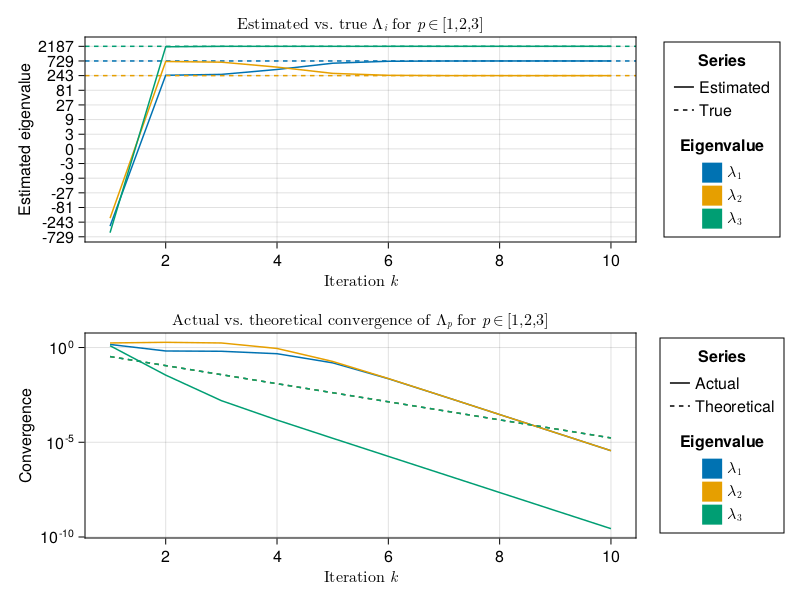
\includegraphics[width=\textwidth]{HW5_code/convergence_final.png}
      \end{center}
      \caption{Eigenvalue convergence for $p = 1, 2, 3$}
      \label{fig:figure1}
    \end{figure}
    \quad Figure \ref{fig:figure1} shows plots of the estimated and true eigenvalues, and the actual and theoretical convergence rates for $p = 1, 2, 3$ and $k \in 1, 2, \dots, 10$.
    Notice that the actual convergence rates are somewhat faster than the theoretical convergence rates.

    \textit{Note: Depending on the generated random matrix, the convergence rates differ between runs.}
    \clearpage
  \subsection*{(d) [10 pts]}
    Consider the block $(p + 1 : m, 1 : p)$ in the matrix 
    \begin{equation}
      \mtx{A}_k = \mtx{Q}^T_{k} \mtx{A} \mtx{Q}_{k}.
    \end{equation}
    Plot the 2-norm of this block as a function of $k$ for $p = 4$. Compare with the analytical estimate, which states that it should decay like $|\lambda_{p + 1} / \lambda_p|^k$.
    
    \begin{figure}[htb]
      \begin{center}
      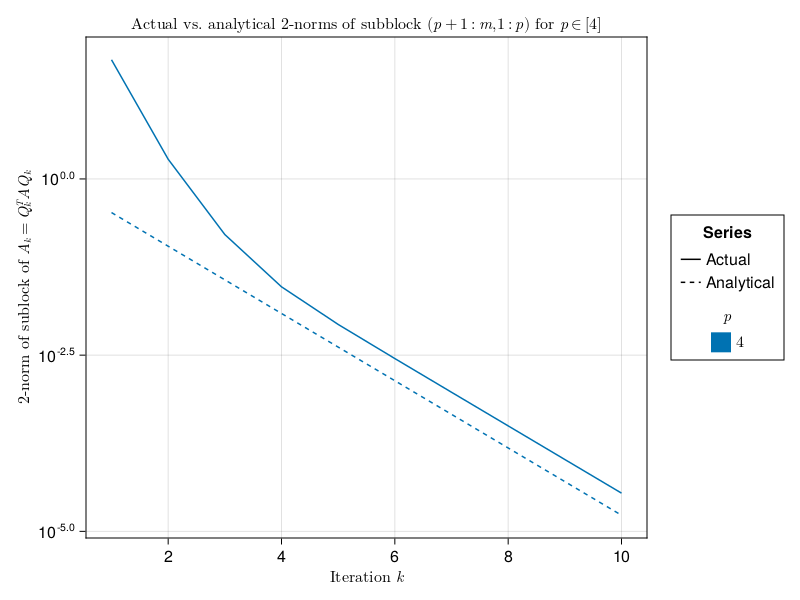
\includegraphics[width=100mm]{HW5_code/norms_final.png}
      \end{center}
      \caption{Analytical vs. actual 2-norm decay rates}
      \label{fig:figure2}
    \end{figure}
    \quad Figure \ref{fig:figure2} shows a plot of the true and analytical 2-norms of these subblocks.
    The analytical norm estimates have exactly the same decay rate as the true norm estimates, though the magnitudes are lower.
  
    \textit{Note: The exact magnitude of the difference in analytic vs true norms is dependent on the generated random matrix.}

\section{LU and QR iteration [20 bonus pts]}
We consider the LU iteration applied to a symmetric matrix. Assume that $\mtx{A}_0 \in \R^{m \times m}$ is symmetric and positive-definite. 
We produce a sequence of matrices $\mtx{A}_i$ using the following algorithm:
\begin{equation}
  \mtx{A}_i = \mtx{G}^T_i \mtx{G}_i, \quad \mtx{A}_{i + 1} = \mtx{G}_i \mtx{G}_i^T, 
\end{equation}
where $\mtx{G}_i$ are upper-triangular matrices.

Consider now $\mtx{A}'$, the matrix obtained after one step of the QR iteration, that is, 
\begin{equation}
  \mtx{A}_0 = \mtx{Q}\mtx{R}, \quad \mtx{A}' = \mtx{R} \mtx{Q}.
\end{equation}
We assume that the diagonal of $\mtx{R}$ is positive.

\subsection*{(a) [10 bonus pts]}
Use $\mtx{A}_0^2$ to show that 
\begin{equation}
  \mtx{R} = \mtx{G}_1 \mtx{G}_0
\end{equation}
\begin{align*}
  \mtx{A}_0^2 &= \mtx{A}_0^2\\
  \mtx{A}_0^T\mtx{A}_0 &= \mtx{A}_0\mtx{A}_0&\text{(since $\mtx{A}$ is symmetric, $\mtx{A} = \mtx{A}^T$)}\\
  (\mtx{Q}\mtx{R})^T(\mtx{Q}\mtx{R}) &= (\mtx{G}^T_0 \mtx{G}_0)(\mtx{G}^T_0 \mtx{G}_0)&\text{(substitute with LU/QR definitions)}\\
  \mtx{R}^T\mtx{R} &= \mtx{G}^T_0 (\mtx{G}_0\mtx{G}^T_0) \mtx{G}_0&\text{(simplify l.h.s., regroup r.h.s.)}\\
  \mtx{R}^T\mtx{R} &= \mtx{G}^T_0\mtx{A}_{1}\mtx{G}_0&\text{(by def. of $\mtx{A}_1$)}\\
  \mtx{R}^T\mtx{R} &= \mtx{G}^T_0(\mtx{G}_1^T\mtx{G}_1)\mtx{G}_0&\text{(by def. of $\mtx{A}_1$)}\\
  \mtx{R}^T\mtx{R} &= (\mtx{G}_1\mtx{G}_0)^T\mtx{G}_1\mtx{G}_0&\text{(rearrange r.h.s.)}\\
  \mtx{R} &= \mtx{G}_1\mtx{G}_0 &\text{(QED)}
\end{align*}

\subsection*{(b) [10 bonus pts]}
Show that
\begin{equation}
  \mtx{A}' = \mtx{A}_2
\end{equation}
\begin{align*}
  \mtx{A}' &= \mtx{A}_2&\text{(given)}\\
  \mtx{A}'^2 &= \mtx{A}_2^2&\text{(square both sides)}\\
  (\mtx{R}\mtx{Q})(\mtx{R}\mtx{Q}) &= (\mtx{G}_1\mtx{G}_1^T)(\mtx{G}_1\mtx{G}_1^T)&\text{(substitute)}\\
  \mtx{R}\mtx{A}_0\mtx{Q} &= \mtx{G}_1\mtx{A}_1\mtx{G}_1^T&\text{(substitute)}\\
  \mtx{R}(\mtx{R}^T\mtx{Q}^T)\mtx{Q} &= \mtx{G}_1\mtx{A}_1\mtx{G}_1^T&\text{($\mtx{A}_0$ is symmetric)}\\
  \mtx{R}\mtx{R}^T &= \mtx{G}_1\mtx{A}_1\mtx{G}_1^T&\text{(simplify l.h.s.)}\\
  (\mtx{G}_1 \mtx{G}_0)(\mtx{G}_1 \mtx{G}_0)^T &= \mtx{G}_1(\mtx{G}_0 \mtx{G}_0^T)\mtx{G}_1^T&\text{($\mtx{A}_{1} = \mtx{G}_0 \mtx{G}_0^T, \mtx{R} = \mtx{G}_1\mtx{G}_0$ (a))}\\
  \mtx{G}_1 \mtx{G}_0\mtx{G}_0^T \mtx{G}_1^T &= \mtx{G}_1\mtx{G}_0 \mtx{G}_0^T\mtx{G}_1^T&\text{(rearrange l.h.s. QED)}\\
\end{align*}

\section{Sensitivity of Eigenvalues [20 bonus pts]}
We are interested in determining the sensitivity of eigenvalues with respect to perturbations in the matrix.

Prove that if $\mtx{A} \in \C^{m \times m}$ is diagonalizable with $\mtx{A} = \mtx{V} \mtx{\Lambda} \mtx{V}^{-1}$, and if $\mu$ is an eigenvalue of $\mtx{A} + \mtx{E}$, 
\begin{equation*}
  \min \limits_{\lambda \in \lambda(\mtx{A})}  \left|\mu -\lambda \right| \leq \kappa_p(\mtx{V}) \|\mtx{E}\|_p.
\end{equation*}
Here $\|\cdot\|_p$ denotes the $p$-norm and $\kappa_p(\mtx{V}) \coloneqq \|\mtx{V}\|_p \|\mtx{V}^{-1}\|_p$ is the condition number associated with the $p$-norm. 

\emph{Hint:} assume that $\Id + \mtx{F}$ is singular. Then, there is an $\vct{x} \neq \vct{0}$ such that $\vct{x} + \mtx{F}\vct{x} = \vct{0}$.
Therefore, $\mtx{F} \vct{x} = -\vct{x}$ and $\|\mtx{F}\|_{p} \geq 1$. 
For the proof, identify the proper singular matrix and use this result. 
\begin{align*}
  (\mtx{A} + \mtx{E})\vct{v} &= \mu\vct{v}&\text{(let $\vct{v}$ be the eigenvector for eigenvalue $\mu$)}\\
  \mtx{A}\vct{v} + \mtx{E}\vct{v} &= \mu\vct{v}&\text{(distribute $\vct{v}$)}\\
  \mtx{V}\mtx{\Lambda}\mtx{V}^{-1}\vct{v} + \mtx{E}\vct{v} &= \mu\vct{v}&\text{(substitute $\mtx{A} = \mtx{V} \mtx{\Lambda} \mtx{V}^{-1}$)}\\
  \mtx{V}\mtx{\Lambda}\vct{c} + \mtx{E}\mtx{V}\vct{c} &= \mu\mtx{V}\vct{c}&\text{(Let $\vct{v} = \mtx{V}\vct{c}$)}\\
  \mtx{V}\mtx{\Lambda} + \mtx{E}\mtx{V} &= \mu\mtx{V}&\text{(drop common $\vct{c}$)}\\
  \mtx{E}\mtx{V} &= (\mu\mtx{I} - \mtx{\Lambda})\mtx{V}&\text{(rearrange)}\\
  \mtx{F} \coloneqq (\mtx{V}^{-1}\mtx{E}\mtx{V}) &= \mtx{V}^{-1}(\mu\mtx{I} - \mtx{\Lambda})\mtx{V}&\text{(left-multiply by $\mtx{V}^{-1}$)}\\
\end{align*}
Observe that $\mtx{I} + \mtx{F}$ is singular.
Thus, there exists a nonzero vector $\vct{x}$ such that
\begin{align*}
  \vct{x} + \mtx{F}\vct{x} &= \vct{0}\\
  \mtx{F}\vct{x} &= -\vct{x}\\
  \|\mtx{F}\|_p &\geq 1&\text{(property of induced matrix norms)}\\
  \|\mtx{V}^{-1}(\mu\mtx{I} - \mtx{\Lambda})\mtx{V}\|_p &\geq 1&\text{(substitute $\mtx{F}$)}\\
  \|\mtx{V}^{-1}\|_p \|\mu\mtx{I} - \mtx{\Lambda}\|_p \|\mtx{V}\|_p &\geq 1&\text{(submultiplicative property of matrix norms)}\\
  \|\mu\mtx{I} - \mtx{\Lambda}\|_p &\geq \frac{1}{\kappa_p(\mtx{V})}&\text{(divide by $ \kappa_p(\mtx{V}) \coloneqq \|\mtx{V}\|_p \|\mtx{V}^{-1}\|_p$)}\\
  \max_{\lambda \in \lambda(\mtx{A})} \left|\mu - \lambda\right| &\geq \frac{1}{\kappa_p(\mtx{V})}&\text{(def. of $p$-norm)}\\
  \min_{\lambda \in \lambda(\mtx{A})} \left|\mu - \lambda\right| &\leq \kappa_p(\mtx{V})&\text{(take the reciprocal of the inequality)}\\
  \min_{\lambda \in \lambda(\mtx{A})} \left|\mu - \lambda\right| &\leq \kappa_p(\mtx{V})\|\mtx{E}\|_p&\text{($\|\mtx{E}\|_p \geq 0$. QED)}
\end{align*}

\end{document}
